\documentclass[11pt,letterpaper]{article}
\usepackage[margin=1in]{geometry}
\usepackage{cite}
\usepackage{amsmath,amssymb,amsfonts}
\usepackage{graphicx}
\usepackage{textcomp}
\usepackage{xcolor}
\usepackage{booktabs}
\usepackage{url}
\usepackage{fancyhdr}
\usepackage{array}
\usepackage{lmodern}
\setlength{\parskip}{0.35em}
\setlength{\parindent}{0pt}
\pagestyle{fancy}
\fancyhf{}
\lhead{ASTRA Technical Report}
\rhead{IASTAM 6.0 -- Track 1}
\cfoot{\thepage}
\setlength{\headheight}{14pt}

\begin{document}

\begin{titlepage}
\centering
\vspace*{1.5cm}
{\Large IEEE IAS Tunisia Annual Meeting (IASTAM 6.0) Technical Challenge\par}
\vspace{1.6cm}
{\huge\bfseries ASTRA\par}
\vspace{0.35cm}
{\LARGE Adaptive Satellite Task and Resource Allocator\par}
\vspace{0.5cm}
{\Large Technical Report: ``Process or Transmit?''\par}
\vspace{1.5cm}
{\large Track 1: Artificial Intelligence and Onboard Computing\par}
\vfill
{\large\bfseries Team Charmoula wMa9rou4\par}
\vspace{0.5cm}
Mohamed Habib Abid\par
\textit{ISI El Manar (Higher Institute of Computer Science), Tunisia}\par
\textrm{mohamedhabib.abid@etudiant-isi.utm.tn}\par
\vspace{0.4cm}
Mariam Neffeti\par
\textit{INSAT (National Institute of Applied Science and Technology), Tunisia}\par
\textrm{mariam.neffeti@insat.ucar.tn}\par
\vfill
{\large 13 October 2026\par}
\end{titlepage}

\section*{Executive Summary}
\addcontentsline{toc}{section}{Executive Summary}
Earth-observation satellites collect data faster than intermittent ground links can routinely return it. Their onboard scheduler must choose whether to process a payload, retain it for later, transmit it during contact, or discard it, while accounting for energy, storage, compute, temperature, data value, and latency. This report presents ASTRA (Adaptive Satellite Task and Resource Allocator), a software research prototype for the IASTAM 6.0 ``Process or Transmit?'' challenge. ASTRA contains a one-second, seeded low-Earth-orbit simulator; transmit-all and greedy edge reference policies; a threshold heuristic; and an exploratory MaskablePPO environment and checkpoint.

The checked-in paired benchmark evaluates four policies over five common-random-number scenarios, each spanning four 90-minute orbits. The threshold heuristic has the highest mean delivered-utility ratio (0.02860; sample standard deviation 0.00142; 95\% Student-$t$ interval [0.02683, 0.03036]). Greedy edge processing completes the greatest fraction of generated payloads (5.17\%), while the heuristic completes 1.60\% and has shorter mean latency among completed deliveries (753 s versus 9,923 s). The single-seed PPO checkpoint delivers no payloads and is not evidence of an operational learned policy. These are synthetic simulator results, not flight measurements. The model uses a linear thermal proxy, and a recorded two-orbit trace reaches 52.48~$^\circ$C despite a 50~$^\circ$C compute-throttling threshold. A Lyapunov scheduler, mixed-integer offline oracle, real telemetry validation, and hard thermal safety layer are not implemented. The report presents ASTRA as an early prototype and measured baseline study, and identifies the work required before safety or generalization claims can be made.

\vspace{0.5em}
\textbf{Keywords:} orbital edge computing; Earth observation; satellite scheduling; energy-aware computing; downlink scheduling; reinforcement learning.

\clearpage
\tableofcontents
\clearpage

\section{Challenge and Objectives}
\subsection{Problem Statement}
The challenge asks for an autonomous decision engine that maximizes the useful scientific and operational value delivered from Earth-observation data under constrained onboard resources and intermittent ground-station visibility. The required decision classes are:
\begin{itemize}
    \item \textrm{PROCESS\_NOW}: run onboard compression or inference to reduce transmitted data or extract an insight;
    \item \textrm{STORE\_QUEUE}: retain a payload or task until resources or contact conditions improve;
    \item \textrm{TRANSMIT\_RAW}: send the unprocessed payload during a ground contact when its full data is warranted; and
    \item \textrm{DISCARD\_DROP}: remove low-utility or unusable data, subject to mission priorities.
\end{itemize}
These choices are coupled. Processing consumes energy and creates heat but can reduce downlink volume. Waiting preserves the option to process or transmit later but occupies finite mass memory and allows utility to decay. Transmission requires line of sight and occupies a short, shared link window. Dropping saves resources but risks losing valuable observations.

\subsection{Project Objectives and Scope}
ASTRA aims to represent orbit, solar generation, battery, payload, storage, compute, thermal, and downlink dynamics in a deterministic, seeded simulator; provide reference policies and an initial learned-policy interface; and compare policies using common environment seeds and resource and outcome metrics. The project distinguishes implemented behavior from assumptions and planned flight-relevant capabilities. This work is a simulator and benchmark study. It does not demonstrate flight readiness, a formally safe controller, or a learned policy that outperforms the baselines.

\section{System Overview}
\subsection{Prototype Architecture}
The implementation separates the simulator from reference policies, the Gymnasium and MaskablePPO interface, and benchmark evaluation and plotting. The simulator owns the physical and workload state; policies read telemetry and request actions; the evaluator runs policies on shared seeds and writes per-episode and summary CSV files.

The separate architecture design describes a future cloud/ground and onboard FaaS system with a model proposal layer, safety guard, fallback, state estimation, and operational logging. These are design targets. The current code does not implement the formally verified guard, cloud orchestration, model-confidence routing, or an atomic persistent journal. Simulator queues and recovery logic are software abstractions, not flight-qualified persistence.

Orbital edge computing motivates moving selected processing closer to the sensor [1], while Trabant describes a serverless architecture for orbital execution [2]. These works provide architectural context; the simulator's numeric workload and resource parameters remain ASTRA assumptions.

\subsection{Assessment Alignment}
The prototype addresses the assessment's resource and orbital constraints through a periodic orbit clock, solar input, battery, thermal proxy, storage, intermittent contact, and decaying utility. It implements several policy classes and produces paired multi-orbit benchmark results. However, orbit and contact geometry remain simplified; parameters and workloads are synthetic rather than calibrated against BUPT-1, Sentinel, VIIRS, or hardware measurements; and Lyapunov and MILP comparisons are absent. The repository has a functional software prototype, not a hardware-in-the-loop or flight demonstration. Thus the implementation shows progress across the assessment areas without claiming that every target is complete.

\section{Simulator and System Model}
\subsection{Orbit, Illumination, and Contact}
The simulation advances in one-second ticks on a 5,400~s (90-minute) orbit. Each orbit contains 3,300~s of modeled sunlight and 2,100~s of eclipse. During sunlight, generated power follows a sinusoidal profile with a 22.5~W base and 7.5~W amplitude, plus 30~s cosine tapers at sunlight boundaries. Generated solar power is zero during eclipse. A randomized ground-station contact begins between 1,000 and 3,000~s into each orbit and lasts 120--180~s. Contacts come from the episode's seeded random stream; this is not a geographic orbit propagator or a ground-station visibility calculation.

These choices approximate the LEO setting but differ from challenge-context examples that use roughly equal sunlight and eclipse, 5--10 minute contacts, and higher peak solar or downlink rates. The benchmark therefore describes the repository's 55/35-minute orbit and 2--3-minute contact model, not every specification scenario. Trace-driven orbital geometry remains future work.

\subsection{Power and Battery}
Default battery capacity is 100~Wh (360,000~J), minimum state-of-charge fraction is 0.30 (108,000~J), and base load is 5~W. Radio draw is 15~W during downlink. Compression draws 10~W; inference draws 20~W while active and 30~W during accelerator wake. The battery integrates the one-second net power balance and caps charging at capacity. If a tick falls below the floor, energy is clamped at the floor and safe mode is entered; safe mode exits above 1.05 times the floor.

The implementation uses unit charge/discharge efficiency and starts episodes with a full battery. It omits battery aging, solar-array degradation, charge-rate limits, and a detailed cell model. The field named \textrm{min\_dod\_fraction} is used as a minimum SoC fraction: it represents a 30\% SoC floor (70\% maximum DoD), not a 30\% maximum DoD.

\subsection{Thermal Model}
The simulator uses a one-node linear temperature proxy:
\begin{equation}
T_{t+1}=T_t+0.15P_t-0.10(T_t-T_{\mathrm{amb}}),
\end{equation}
where power includes base, compute, and communication draw, and default ambient temperature is 0~$^\circ$C. At or above 50~$^\circ$C, processing is throttled. This is not the Stefan--Boltzmann radiation balance required for a physically grounded vacuum model, and the threshold is not a hard temperature bound: transient temperature can exceed it. The documented seed-42, two-orbit trace peaks at 52.48~$^\circ$C. The current model therefore cannot support a claim that ASTRA maintains a strict 50~$^\circ$C safety invariant.

\subsection{Payload, Compute, and Utility}
The simulator creates one payload every 15~s. Modality is synthetic: optical with probability 0.70, or SAR with probability 0.30. Optical payload sizes range from 5 to 15~MB; SAR sizes range from 100 to 300~MB. Base values are drawn uniformly from 10 to 100, with optical value scaled by one minus a random cloud fraction. Utility decays exponentially with age:
\begin{equation}
U_k(t)=U_{0,k}\exp[-\alpha_k(t-t_k)],\qquad
\alpha_k\in[10^{-4},10^{-3}]~\mathrm{s}^{-1}.
\end{equation}
Compression takes 2~s at 10~W and reduces payload size to 30\% while retaining 90\% of value. Inference takes 5~s at 20~W after a 2~s, 30~W wake period; it reduces payload size to 0.1\% while retaining 50\% of value. A serial processing queue holds at most four jobs. These ratios, values, cloud distributions, and rates are synthetic parameters, not measured CNN benchmarks or validated satellite telemetry.

\subsection{Storage, Fault Abstraction, and Downlink}
Default mass-memory capacity is 32,000~MB and RAM is 4,000~MB. Payloads queued for processing remain accounted against mass memory until processing completes; RAM holds a working copy of the active job. A per-second Bernoulli event with configured probability $10^{-5}$ resets RAM and accelerator state; queued work is recovered to mass memory by the simulator. This SEU proxy does not model radiation transport, bit-level corruption, or hardware reboot validation. No SEUs occurred in the five paired evaluation episodes, which provides little evidence about rare-event behavior.

The modeled downlink rate is 20~Mbps (2.5~MB/s), with a 15~W radio draw. Transmission requires a ground-station pass and uses a shared per-tick bandwidth budget. The model omits link margin, coding overhead, packet loss, protocol overhead, weather, pointing, antenna acquisition, and geographic visibility traces.

\section{Decision Policies and Learning Setup}
\subsection{Reference Policies}
\begin{table*}[t]
\caption{Implemented Policies and Their Interpretation}
\label{tab:policies}
\centering
\small
\begin{tabular}{p{0.15\textwidth}p{0.48\textwidth}p{0.29\textwidth}}
\toprule
\textbf{Policy} & \textbf{Implemented behavior} & \textbf{Purpose and interpretation}\\
\midrule
Transmit-all & Sends the oldest raw mass-memory payload during contact; no processing or voluntary drop. & Conventional bent-pipe reference.\\
Greedy-edge & Processes the oldest eligible payload whenever queue capacity permits; downlinks processed payloads during contact. & Immediate-processing reference.\\
Threshold heuristic & During contact, ranks payloads by processed status and current value for downlink; processes when SoC $>0.5$, not throttling, and queue length $<2$; drops low-value data when MMU exceeds 80\%. & Current ASTRA rule-based baseline.\\
MaskablePPO & Uses telemetry and up to five payload slots with invalid-action masks; checkpoint trained with seed 7. & Exploratory diagnostic only.\\
\bottomrule
\end{tabular}
\end{table*}

These baselines are operational comparison definitions, not optimized implementations. Greedy edge does not use a separate design-level safety supervisor. Heuristic thresholds are implementation rules rather than derived optimal thresholds.

\subsection{PPO Environment}
The Gymnasium environment provides normalized system telemetry and metadata for a top-$K$ payload set. Each of five slots can request no action, compression, inference, downlink, or drop. Invalid-action masks exclude actions considered unavailable in the current state. Reward uses newly delivered utility, penalties for voluntary and involuntary drops, and safe-mode entry, plus a small shaped reward for accepted processing actions to address delayed utility realization at downlink.

Checkpoint metadata records training seed 7 and 100,352 actual training steps (100,000 requested). The checkpoint is evaluated deterministically on disjoint environment seeds. A single training seed cannot characterize variability across training runs. Its zero-delivery result is a failure of this checkpoint under the reported evaluation, not evidence that reinforcement learning as a class is inferior.

\subsection{Unimplemented Benchmark Targets}
The challenge hierarchy calls for an online Lyapunov or other dynamic scheduler and an offline oracle, such as a MILP with future knowledge. Neither is implemented in this repository snapshot. The learned policy does not substitute for these missing comparisons, and no result relative to an oracle or Lyapunov policy is claimed. Prior work on stochastic network optimization motivates such online scheduling approaches \cite{neely}.

\section{Evaluation Method}
Four policies are evaluated on five common seeds (1001--1005), each for four orbits, or 21,600 one-second steps. The same seed gives each policy the same generated payloads, station windows, and SEU draws, enabling paired comparison. The results include per-policy means, sample standard deviations, and two-sided 95\% Student-$t$ intervals with four degrees of freedom. Paired-difference outputs report episode-wise differences relative to the heuristic.

Metrics include: (i) decision quality, delivered utility divided by the sum of generated payload base values; (ii) completed-task rate, fully downlinked payloads divided by generated payloads; (iii) cumulative modeled base, compute, and radio energy; (iv) mean capture-to-completion latency for completed deliveries; (v) time-average MMU and RAM occupancy as a percentage of capacity; and (vi) SEU and safe-mode event counts per episode.

The decision-quality denominator is a base-value snapshot and does not adjust for value retained after processing. Latency is conditional on completed deliveries; when few payloads complete, its mean may be misleading. Metrics should be read together. Five scenarios provide preliminary uncertainty estimates, not strong generalization or rare-event evidence. PPO training-seed variability is not measured.

\section{Results}
\subsection{Primary Comparison}
Table~\ref{tab:results} reports the checked-in benchmark means, sample standard deviations, and 95\% intervals.

\begin{table*}[t]
\caption{Paired Policy Comparison Across Five Four-Orbit Episodes (Mean; Sample SD; 95\% Student-$t$ Interval)}
\label{tab:results}
\centering
\scriptsize
\resizebox{\textwidth}{!}{%
\begin{tabular}{lcccc}
\toprule
\textbf{Metric} & \textbf{Transmit-all} & \textbf{Greedy-edge} & \textbf{Heuristic} & \textbf{MaskablePPO (seed 7)}\\
\midrule
Decision quality & .00183; .00115; [.00040,.00326] & .00470; .00105; [.00339,.00601] & \textbf{.02860; .00142; [.02683,.03036]} & 0; 0; [0,0]\\
Completed-task rate & 1.57\%; .21\%; [1.31\%,1.83\%] & \textbf{5.17\%; .80\%; [4.17\%,6.17\%]} & 1.60\%; .05\%; [1.54\%,1.66\%] & 0; 0; [0,0]\\
Energy & 117.15; .34; [116.73,117.57] kJ & 290.88; 1.76; [288.70,293.07] kJ & 290.88; 1.76; [288.70,293.07] kJ & 206.01; 4.78; [200.07,211.95] kJ\\
Delivery latency & 9,659; 1,996; [7,181,12,136] s & 9,923; 1,290; [8,322,11,524] s & \textbf{753; 121; [603,904] s} & N/A (no delivery)\\
Mean MMU utilization & 82.81\%; 1.96\%; [80.39\%,85.24\%] & 38.16\%; 1.91\%; [35.79\%,40.54\%] & 37.96\%; 1.90\%; [35.60\%,40.32\%] & 48.77\%; 3.63\%; [44.27\%,53.28\%]\\
Mean RAM utilization & 0 & .173\%; .003\%; [.169\%,.177\%] & .173\%; .003\%; [.169\%,.177\%] & .439\%; .036\%; [.394\%,.484\%]\\
SEU events per episode & 0 & 0 & 0 & 0\\
Safe-mode events per episode & 0 & 0 & 0 & 0\\
\bottomrule
\end{tabular}%
}
\end{table*}

\subsection{Interpretation}
The threshold heuristic delivered the largest fraction of generated base utility and had the shortest average latency among completed deliveries. Greedy-edge completed the most payloads, but its delivered-utility ratio was lower. Completion rate alone therefore does not measure scientific value. Transmit-all used the least modeled energy but accumulated high memory occupancy and long delivery latency under this synthetic workload and contact schedule.

Greedy-edge and heuristic have identical per-seed aggregate energy in this experiment. This is a property of the observed run and model accounting, not a general equivalence between the policies; their task selections and delivery outcomes differ.

The PPO checkpoint completed no tasks in any evaluation episode. Its lower energy than the two processing-heavy policies is not an efficiency gain because it delivered no utility; it also used more energy than transmit-all. This result motivates further reward, training, and action-selection investigation.

No SEU or safe-mode events occurred in the paired benchmark. A separate heuristic telemetry trace has SoC between 92.37\% and 100\% and temperature peaking at 52.48~$^\circ$C. Zero observed events over five episodes do not establish fault tolerance or safety. The thermal trace confirms that the current throttle is not a strict temperature cap.

\begin{figure}[t]
\centering
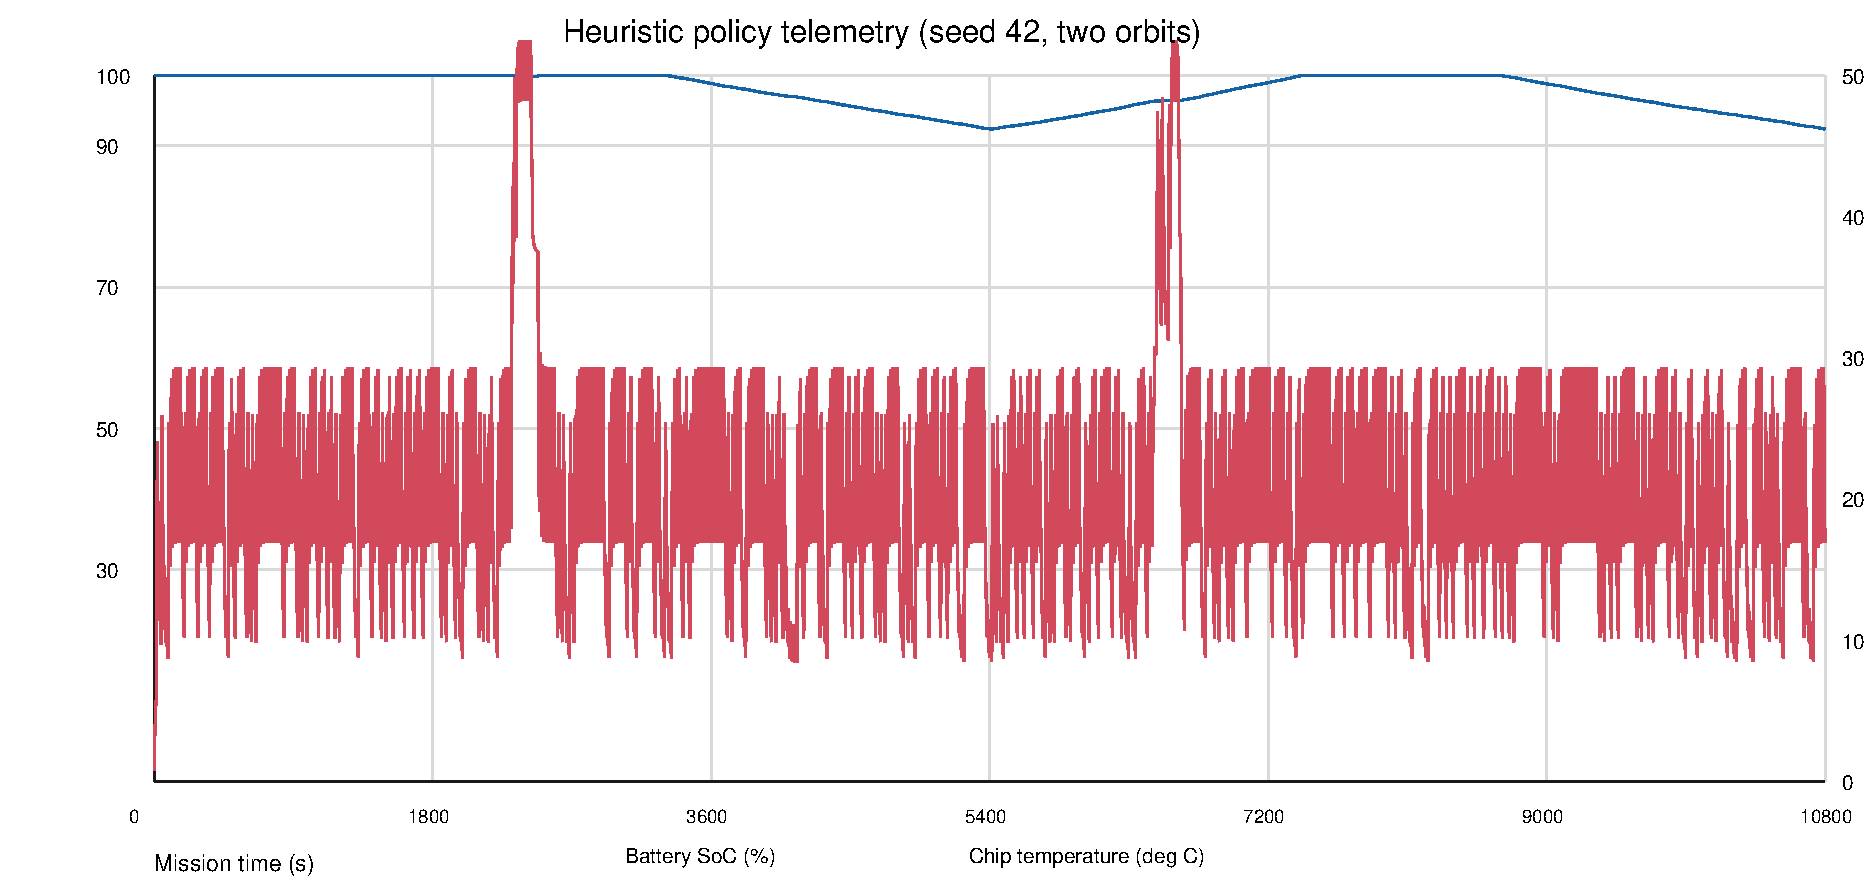
\includegraphics[width=\columnwidth]{../../results/figures/orbit_telemetry.pdf}
\caption{Heuristic telemetry over two orbits (seed 42). Temperature exceeds the 50~$^\circ$C throttle threshold.}
\label{fig:telemetry}
\end{figure}

\begin{figure}[t]
\centering
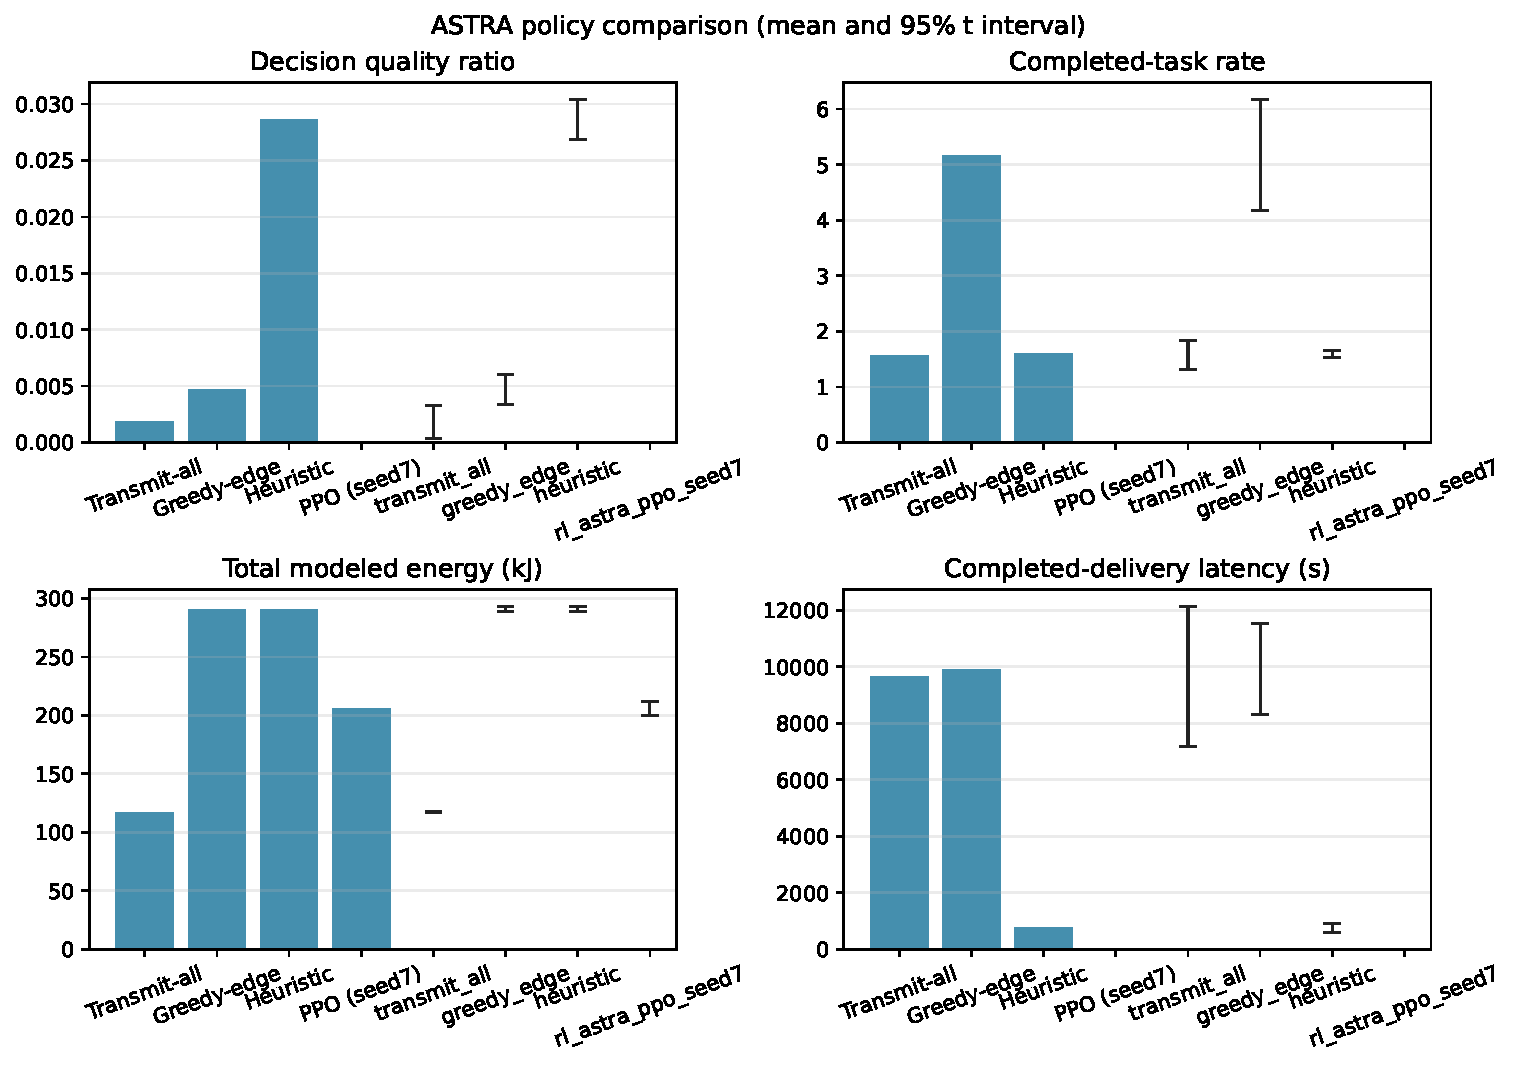
\includegraphics[width=\columnwidth]{../../results/figures/policy_comparison.pdf}
\caption{Policy comparison across five paired episodes. PPO completes no tasks in this run.}
\label{fig:comparison}
\end{figure}

\section{Limitations and Validity}
\begin{enumerate}
    \item \textbf{Synthetic scenario:} Workload, values, cloud cover, station contacts, and processing ratios are generated from simulator parameters. No real observation or telemetry trace is replayed.
    \item \textbf{Simplified orbit:} The periodic clock uses fixed illumination and randomized contacts. It does not calculate orbital position, beta angle, station elevation, or contact geometry.
    \item \textbf{Thermal safety gap:} The linear proxy and throttle do not enforce a hard temperature bound; a recorded trace exceeds 50~$^\circ$C.
    \item \textbf{Simplified energy:} The battery starts full; charge/discharge efficiency and degradation are omitted. Safe-mode decisions may follow actions already applied in that tick.
    \item \textbf{SEU abstraction:} The random reset does not model radiation dose, bit-level corruption, or hardware recovery. Five episodes with zero events do not evaluate rare-event robustness.
    \item \textbf{Small sample:} Five evaluation seeds are preliminary, and one PPO training seed provides no estimate of training variability.
    \item \textbf{Metric interpretation:} Decision quality uses generated base value; latency is calculated only for completed deliveries. Both metrics have selection and retention effects.
    \item \textbf{Missing references:} No Lyapunov policy or non-causal MILP upper bound is available, so the full required benchmark hierarchy is not evaluated.
    \item \textbf{Reproducibility workflow:} Defaults are in \textrm{SimConfig}; the \textrm{configs/} directory does not yet load external YAML configuration files.
\end{enumerate}

\section{Conclusions and Completion Plan}
ASTRA establishes a modular, seeded simulator and a first paired comparison of conventional transmission, immediate edge processing, a resource-aware heuristic, and an initial learned policy. In this experiment, the heuristic leads on delivered utility and completed-delivery latency; greedy edge leads on completion fraction; and the PPO checkpoint delivers no tasks. These findings are limited to a small synthetic benchmark and do not establish flight performance or safety. A measured temperature excursion above the throttle threshold, missing oracle and Lyapunov comparisons, and lack of real telemetry validation are material gaps.

The next work should prioritize: (1) replacing or calibrating the thermal proxy and adding an independent action safety guard; (2) adding cited, configurable orbital, power, and contact scenarios; (3) implementing Lyapunov and non-causal MILP comparisons under common assumptions; (4) expanding held-out episodes and evaluating multiple PPO training seeds; (5) validating workload and hardware assumptions against public traces or hardware-in-the-loop measurements; (6) adding fault-injection and persistent-state recovery evidence; and (7) confirming final author metadata, references, and submission formatting.

\begin{thebibliography}{00}
\bibitem{denby} B. Denby and B. Lucia, ``Orbital Edge Computing: Machine Inference in Space,'' \textit{IEEE Computer Architecture Letters}, vol. 18, no. 1, pp. 59--62, Jan.--Jun. 2019, doi: 10.1109/LCA.2019.2907539.
\bibitem{trabant} T. Pfandzelter et al., ``Trabant: A Serverless Architecture for Multi-Tenant Orbital Edge Computing,'' arXiv:2504.08337, 2025.
\bibitem{neely} M. J. Neely, \textit{Stochastic Network Optimization with Application to Communication and Queueing Systems}. Morgan \& Claypool Publishers, 2010.
\end{thebibliography}

\end{document}
